\documentclass[10pt]{gshs-report-v2.0}
% 추가로 필요한 패키지가 있다면 이곳에 적어 넣으시오.
\usepackage{enumitem}
\usepackage{multirow}
\usepackage{cite}
\usepackage{bm}
\usepackage{makecell}

\usepackage{amsmath, amsfonts, amsthm, amssymb}
\usepackage[utf8]{inputenc}
\usepackage[english]{babel}
\usepackage{hyperref}
\usepackage[capitalize,nameinlink]{cleveref}
\usepackage{graphicx, wrapfig}
\usepackage{caption, subcaption}
\usepackage{verbatim, listings, fancyvrb}

\theoremstyle{theorem}
\newtheorem{theorem}{Theorem}[section]
\theoremstyle{lemma}
\newtheorem{lemma}[theorem]{Lemma}
\theoremstyle{definition}
\newtheorem{definition}[theorem]{Defintion}

\hypersetup{
	colorlinks=true,
	linkcolor=black,
	citecolor=blue,
	urlcolor=cyan,
}

%%%%%%%%%%%%%%%%%%%%%%
%%%%%알앤이 정보%%%%%%
%%%%%%%%%%%%%%%%%%%%%%

%사업 시행 년도
\researchYear{2021}

%연구 종류: 기초 또는 심화
\researchtype{심화} 

%보고서 종류: 중간 또는 최종
\reporttype{최종} 


% 제목 및 영문 제목: 개행 시에는 \linebreak만 사용 가능하다.
\title{베지어 곡면을 이용한 3D 모델링} 
\englishtitle{Application of Bézier Curve to 3D Modeling}

% 제출 년월일
\summitdate{2021}{12}{24}

%연구 참여자 (저자 1, 2, 3)
\author[1]{박건호}
\email[1]{abc0004@naver.com}
\author[2]{윤상}
\email[2]{abc0004@naver.com}

%연구 책임자: 없는 경우 그대로 내버려 둘 것, 있는 경우 채울 것
\professor{}
\professorEmail{abc0004@naver.com}

%지도교사
\advisor{김소연}
\advisorEmail{abc0004@naver.com}




\graphicspath{{figures/}}
\renewcommand{\contentsname}{차례}
\renewcommand{\listfigurename}{그림 목차}
\renewcommand{\figurename}{그림}
\renewcommand{\tablename}{표}
\setlength{\tabcolsep}{10pt}
\renewcommand{\arraystretch}{1.5}


%%%%%%%%%%%%%%%%%%%%%%%%%%
%%%%%%%%문서 시작%%%%%%%%%
%%%%%%%%%%%%%%%%%%%%%%%%%%
\begin{document}


%%%%%%%%%%%%%%%%%%%%%%
%%%%%제목 페이지%%%%%%
%%%%%%%%%%%%%%%%%%%%%%
\makecover


%%%%%%%%%%%%%%%%%%%%%%%%%%%%%
%%%%%요약문(국문) 페이지%%%%%
%%%%%%%%%%%%%%%%%%%%%%%%%%%%%
\noindent{
\huge 베지어 곡면을 이용한 3D 모델링
}\\
\vspace{10pt}
\noindent{
\Large Application of Bézier Curve to 3D Modeling
}

\setstretch{1.6}
\begin{abstractkor}
\noindent{
공학 설계를 하는 CAGD 분야에서 자동차 차체, 비행기 기체 등을 설계하는 과정에서 베지어 곡면이라는 특수한 곡면을 많이 사용한다. 이렇게 베지어 곡면을 많이 사용하는 이유는 베지어 곡면은 삼각형 분할에 비해 부드러운 곡면을 표현함에 더 강하고, 적은 메모리를 필요로 한다는 장점이 있기 때문이다. 우리 연구에서는 베지어 곡면을 이용해 obj파일로 주어진 3D 모델을 근사하고 압축하는 방법을 다룬다. 이 연구는 3차원 공간상의 볼록 집합의 경계를 대상으로 하며 기존의 베지어 곡면을 이용한 point cloud(물체의 나타내는 점들)의 근사 방법을 확장해 연구했다. 고차 베지어 곡면도 활용성이 높지만 고차 베지어 곡면은 다루기 까다롭기에 (2,2)차 베지어 곡면을 이용하였으며, 이를 효율적으로 근사하기 위해 point cloud를 원통형으로 분할하는 과정을 거쳤다. 분할한 각 영역의 점들을 하나의 베지어 곡면으로 근사하였고, 광선과 삼각형의 교점을 찾는 Möller–Trumbore intersection algorithm과 선행 연구를 참고해 최소제곱법, 뉴턴-랩슨 방법을 사용하여 최대한 빠른 시간안에 근사가 되도록 하였다. 베지어 곡면과 원 곡면의 차이를 나타내는 즉, 잘 근사되었는지 나타내주는 오차함수는 하우스도르프 거리가 적합하지만, 계산량이 너무 많은 단점 때문에 적절히 변형해 새로운 오차함수를 만듦으로서 적은 시간을 소모하게 만들었다. 더 나아가 엡실론-델타 논법을 이용해 곡면들이 충분히 근사 가능함을 수학적으로 증명하였다. 본 연구를 통해 곡면 모델링이 핵심이 되는 VR, AR 및 홀로그램의 컴퓨터 그래픽 분야에서의 활용이 기대된다. 또한 CAGD 분야에서 더 큰 활용이 가능하며 이에 따라 자동차, 선박, 비행기 뿐만 아니라 미래 우주 공학과도 직결되는 우주선이나 우주 정거장을 디자인하는 데도 사용될 수 있다.
}
\end{abstractkor}
%요약문 관련 팁: 요약문은 가장 마지막에 작성한다. 연구한 내용, 즉 본론부터 요약한다. 서론 요약은 하지 않는다. 대개 첫 문장은 연구 주제 (+방법을 핵심적으로 나타낼 수 있는 문구: 실험적으로, 이론적으로, 시뮬레이션을 통해)를 쓴다. 다음으로 연구 방법을 요약한다. 선행 연구들과 구별되는 특징을 중심으로 쓴다. 뚜렷한 특징이 없다면 연구방법은 안써도 상관없다. 다음으로 연구 결과를 쓴다. 연구 결과는 추론을 담지 않고, 객관적으로 서술한다. 마지막으로 결론을 쓴다. 이 연구를 통해 주장하고자 하는 바를 간략히 쓴다. 요약문 전체에서 연구 결과와 결론이 차지하는 비율이 절반이 넘도록 한다. 읽는 이가 요약문으로부터 얻으려는 정보는 연구 결과와 결론이기 때문이다. 연구 결과만 레포트하는 논문인 경우, 결론을 쓰지 않는 경우도 있다.

\pagebreak

%%%%%%%%%%%%%%%%%%%%%%%%%%%%%%%%%%
%%%%%목차, 표 목차, 그림 목차%%%%%
%%%%%%%%%%%%%%%%%%%%%%%%%%%%%%%%%%
\tableofcontents
\pagebreak
\listoffigures
%\listoftables
\pagebreak

\pagenumbering{arabic}
\setcounter{page}{1}

%%%%%%%%%%%%%%%%%%%%%%%%%%
%%%%%%%%본문 시작%%%%%%%%%
%%%%%%%%%%%%%%%%%%%%%%%%%%

\section{서론}

\subsection{연구 필요성 및 목적}
3D 프린터, 홀로그램 및 VR과 AR은 지금도 활발하게 사용되고 있는 기술이고 앞으로도 많은 사람이 관심을 가질 분야이다. 이들이 실제로 상용화되기 위해서는 더 효율적으로 곡면을 다루기 위한 컴퓨터 그래픽 기술 특히 메모리로 인한 처리 시간을 줄이는 기술이 필수적이다. 

현재 3D 모델은, 저장, 프로그램 사용 등 많은 부분에서 대부분 obj파일 형식으로 사용된다. obj파일의 f 부분을 보면 곡면을 표현하기 위해 삼각형 혹은 사각형 분할을 이용한다는 것을 알 수 있다. 이러한 다각형 분할은 많은 장점이 있지만 베지어 곡면을 이용한 압축에 비해 구면과 같은 부드러운 곡면을 표현하는 능력이 떨어진다는 단점도 있다. 또한 베지어 분할은 베지어 곡면이 가지는 조절점이라는 고유한 성질 덕에 메모리도 적게 소모되어 더 효율적일 것이다. 

본 연구는 obj파일 형식으로 주어진 3차원 공간상의 곡면을 조각별로 분할하여 베지어 곡면을 통해 근사 및 압축하는 방법을 제시한다. 이는 obj파일에 비해 메모리 측면에서의 이점을 가진다. 혹은 자동차, 선박, 비행기 등을 설계할 때 이용되는 CAD(Computer Aided Design) 중에서도 수학적인 도구를 이용하는 CAGD 분야에서의 활용이 기대된다. 

\subsection{이론적 배경}
\subsubsection{베지어 곡선과 곡면}
\begin{definition} \label{BC}
	\textbf{$\boldsymbol{n}$차 베지어 다항식(Bézier polynomial)}은 $n+1$개의 점 $\mathbf{P}_0, \mathbf{P}_1, \cdots, \mathbf{P}_n$에 대해 다음과 같이 주어진다.
	\begin{equation}
		\mathbf{B}(t)=\sum_{i=0}^n \binom ni(1-t)^{n-i}t^i\mathbf{P}_i
	\end{equation}

	이때 $n$차 베지어 다항식에 의한 폐구간 $[0, 1]$의 상을 \textbf{$\boldsymbol{n}$차 베지어 곡선(Bézier curve)}이라 한다. 또한 점 $\mathbf{P}_0, \cdots, \mathbf{P}_n$을 이 베지어 곡선의 \textbf{조절점(control point)}이라 한다. 
\end{definition}

편의상 베지어 곡선을 BC로 표기하자.

\begin{definition} \label{BS}
	$(n+1)(m+1)$개의 점 $\mathbf{b}_{ij}\ (i=0, 1, \cdots, n\ \mathrm{and}\ j=0, 1, \cdots, m)$에 대해 다음 $2$변수 다항식을 생각하자. 
	\begin{equation}
		\mathbf{x}(u, v)=\sum_{i=0}^n\sum_{j=0}^m B_i^n(u)B_j^m(v)\mathbf{b}_{ij} 
	\end{equation}
	
	여기서 Bernstein 다항식 $B_i^n(t)=\binom ni(1-t)^{n-i}t^i$로 주어진다. $\mathbf{x}$에 의한 단위 정사각형 $[0, 1]^2$의 상을 \textbf{$\boldsymbol{(n, m)}$-차 베지어 곡면(Bézier surface)}이라 한다. 마찬가지로 점 $\mathbf{b}_{ij}$를 이 베지어 곡면의 조절점이라 한다.\cite{Farin}
\end{definition}

\begin{figure}[h]
	\centering
	\begin{subfigure}[b]{.45\textwidth}
		\centering
		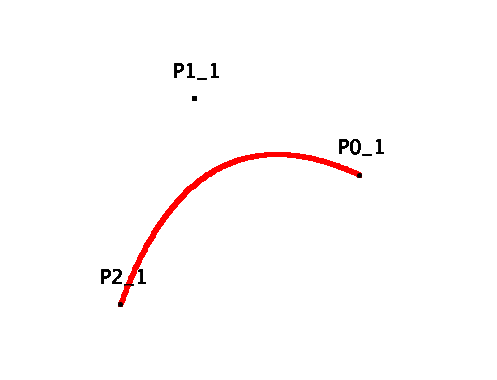
\includegraphics[width=\textwidth]{BC}
		\caption{베지어 곡선}
	\end{subfigure}
	\hfill
	\begin{subfigure}[b]{.45\textwidth}
		\centering
		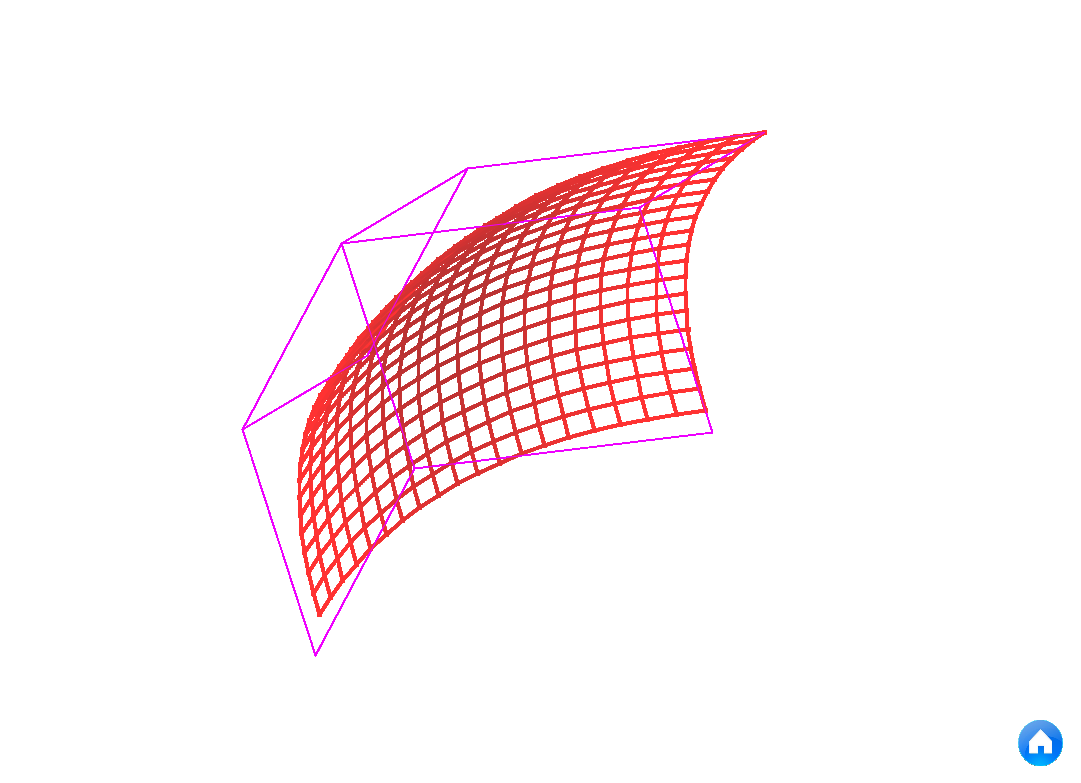
\includegraphics[width=\textwidth]{BS}
		\caption{베지어 곡면}
	\end{subfigure}
	\caption{베지어 곡선(a)과 베지어 곡면(b)}
\end{figure}

\subsubsection{볼록 집합}
\begin{definition}
	$\mathbb{R}^n$의 부분집합 $C$가 다음 조건을 만족할 때, $C$를 \textbf{볼록 집합(convex set)}이라 부른다. 
	\begin{equation*}
		\forall \mathbf{x}, \mathbf{y} \in C,\ \forall t \in [0, 1],\ (1-t)\mathbf{x}+t\mathbf{y} \in C
	\end{equation*}
\end{definition}

\begin{theorem} \label{homeo}
	$\mathbb{R}^n$의 볼록 집합 $C$의 내부(interior)가 공집합이 아닐 때, $C$의 경계(boundary) $\partial C$는 $S^{n-1}$과 위상동형이다. 여기서 $S^{n-1}$은 $(n-1)$차원 단위 구면으로, $S^{n-1}=\{ \mathbf{x}\in\mathbb{R}^n \mid \| \mathbf{x} \| = 1 \}$이다.
\end{theorem}

간단히 증명하면, $C$의 내부가 공집합이 아니므로 $C$를 평행이동하여 $\mathbf{0}\in C^\circ$가 되도록 만들 수 있다. 이제 함수 $f\colon\partial C \to S^{n-1}$을 $f(\mathbf{x})=\mathbf{x}/\|\mathbf{x}\|$로 정의하면 $f$는 위상동형사상이 된다. 

\subsubsection{뉴턴-랩슨 방법}
뉴턴-랩슨 방법은 미분가능한 실수값 함수의 근을 찾는 알고리즘이다. 함수 $f\colon(a, b)\to\mathbb{R}$과 도함수 $f^\prime$에 대해, 현재 $f(x)=0$의 해의 근사치를 $x_n$이라 하자. $f$의 선형 근사는 다음과 같다.
\begin{equation*}
	y=f^\prime(x_n)(x-x_n)+f(x_n)
\end{equation*}

다음 근사치 $x_{n+1}$은 위 직선의 $x$절편으로 주어진다.
\begin{equation} \label{newton}
	x_{n+1}=x_n-\frac{f(x_{n})}{f^\prime(x_n)}
\end{equation}

초기값 $x_0$부터 시작해 \cref{newton}을 반복해 더 좋은 근사치를 얻을 수 있다. 그러나 초기값의 선택에 따라 $\{x_n\}$이 발산할 수 있다. 그리고 $f$가 근을 가지지 않는다면 국소 최솟값을 얻는다.

\subsubsection{obj와 mtl}
obj는 3D 이미지를 저장하는 표준적인 파일이다. obj는 3차원 물체를, mtl은 3차원 물체의 색상, 재질, 반사도 등을 저장한다. 일반적으로 프로그램을 통해 3차원 모델을 만들면 obj와 mtl 파일이 모두 만들어진다. 

우선 obj 파일은 정점 $v$, 단위 법선벡터 $v_n$, 텍스쳐 $v_t$, 면 $F$로 이루어진다. 먼저 $v, v_n, v_t$의 $x, y, z$성분이 차례로 주어진다. 마지막에 $F$가 주어지는데, 각각의 $F$는 $v/v_n/v_t$ 블록 3개 또는 4개로 이루어진다. 3개면 삼각형 면, 4개면 사각형 면이다. 아래는 obj 파일의 예시이다. 
\begin{Verbatim}
# object heart

v -5.7868 -2.8897 6.9550
v -5.8939 -2.7443 6.7745
...
v 1.3498 1.7948 1.8726
# 5636 vertices

vn -0.3934 -0.8264 -0.4029
...
vn 0.2663 0.7947 -0.5454
# 5634 vertex normals

vt 0.1020 0.1559 0.0000
...
vt 0.7205 0.0233 0.0000
# 5974 texture coordinates

g Heart       # o [object name] / g [group name] 
usemtl Heart  # usemtl [material name]
s 1           # s : smooth
f 1/1/1 2/2991/2 3/1583/3 4/2994/4
...
f 5598/1580/5598 5595/5955/5595 5634/2990/5634 5633/5974/5633
\end{Verbatim}

mtl은 ambient 반사도 $K_a$, diffuse 반사도 $K_d$, specular 반사도 $K_s$ 등으로 이루어진다. 모두 0에서 1 사이의 값을 가지며 각각 물체가 원래 가지고 있는 색에 의한 반사도, 국소적인 색에 의한 반사도, 하이라이트를 일으키는 반사도를 의미한다. 본 연구에서는 $K_a$ 및 $K_d$만 사용했다. 

\section{연구 과정}

\subsection{연구 질문}
연구 질문은 다음과 같다:
\begin{enumerate}
	\item point cloud가 주어졌을 때 베지어 곡면을 이용해 점들을 충분히 근사할 수 있다. (i.e. 오차함수가 0으로 수렴한다)
	\item obj 등 기존의 곡면을 저장하는 방식보다 더 높은 압축 효율을 가진다.
	\item 기존 mtl과 같이 곡면이 지닌 색, 질감 등의 성질도 베지어 곡면의 특징을 이용해 압축하여 저장할 수 있다.
	\item 근사하거나 구현하는 과정에서 시간이 obj보다 적게 소모된다.
	\item 적절한 오차함수를 정의해 근사 정도를 확인하고 기존의 방법보다 오차가 적음을 보인다. 
\end{enumerate}

\subsection{분할 방법}
주어진 모델을 하나의 베지어 곡면으로 나타내려면 오차가 너무 커진다. 그래서 우리는 obj 파일의 정점 혹은 point cloud를 분할하고, 분할된 각 영역의 곡면을 하나의 베지어 곡면으로 근사하는 방법을 택했다. 이를 위해 고안한 두 가지 분할 방법이 있다. 

\begin{itemize}
	\item \textbf{8진 트리.} 8진 트리는 카테시안 좌표계를 기준으로 하며, 원점(기준점)에 대해 공간을 $xy$평면, $yz$평면, $zx$평면으로 잘라 8개의 영역으로 나누는 방식이다. 8개 영역으로 분할되기 때문에 8개의 자식 노드가 생긴다고 볼 수 있다. 8진 트리 방식의 장점은 모델의 제한 없이 항상 적용 가능하다는 점이다. 그러나 분할된 조각을 베지어 곡면으로 근사하기 어렵고, 조각이 8배씩 많아지므로 시간이 오래 걸린다.
	
	\item \textbf{원통형 분할.} 원통형 분할은 원통형 좌표계를 기준으로 하며, $(r, \theta, z)$로 표현되는 정점들을 $\theta$와 $z$에 따라 나눈다. $\theta-z$ 평면에 각 정점들을 표현하고 $4^n$등분하여 영역을 분할하는 방식이다. 원통형 분할은 같은 $(\theta, z)$ 값에 대해 두 개 이상의 점이 존재하면 적용할 수 없다는 단점이 있다. 그러나 8진 트리 방법보다 시간이 적게 소모되고, 최종적으로 만들어진 곡면을 조각적으로 정의된 연속함수 $\mathbf{x}^*\colon\mathbb{R}^2\to\mathbb{R}^3$에 대해 $\mathbf{x}^*([0, 1]^2)$으로 표현할 수 있다는 장점이 있다. 이 점은 모델의 RGB 색을 압축할 때도 사용될 수 있다. 
\end{itemize}

우리는 원통형 분할을 이용하기로 결정했다. 또한 위에서 설명한 단점을 없애기 위해 연구 대상을 축소했다. $\mathbb{R}^3$의 볼록 집합의 경계로 표현되는 곡면만을 근사한다. \cref{homeo}에 따라 이는 2차원 곡면이 된다. 

\subsection{근사 방법}
분할된 곡면을 근사하는 베지어 곡면을 결정하기 위해서 9개의 조절점이 필요하다. 결정된 베지어 곡면이 연속적으로 이어지기 위해서는 $\mathbf{b}_{11}$를 제외한 나머지 조절점은 영역 안에 있는 정점들과는 무관하게 결정되어야 한다. 각 영역의 경계는 $\theta=\theta_i$ 혹은 $z=z_j$로 주어지므로, 직선 $\ell \colon \theta=\theta_i, z=z_j$와 obj 파일의 면 $F$의 교점으로 네 조절점 $\mathbf{b}_{00}, \mathbf{b}_{02}, \mathbf{b}_{20}, \mathbf{b}_{22}$를 구한다. 여기서 직선과 삼각형의 교점을 찾는 빠른 알고리즘인 Möller-Trumbore intersection algorithm을 사용한다.\cite{raytriangle} 그리고 작년 연구를 활용하면 다시 네 조절점 $\mathbf{b}_{01}, \mathbf{b}_{10}, \mathbf{b}_{12}, \mathbf{b}_{21}$을 얻을 수 있다. (2,2)차 베지어 곡면에서, $u=0,\ u=1,\ v=0,\ v=1$인 부분은 각각 2차 베지어 곡선이 되기 때문이다. 두 영역의 경계 $\theta=\theta_i, z\in[z_j, z_{j+1}]$ 혹은 과 $F$들의 교선을 하나의 2차 베지어 곡면으로 근사하면 된다.\cite{last year} 

\begin{figure}[h]
	\centering
	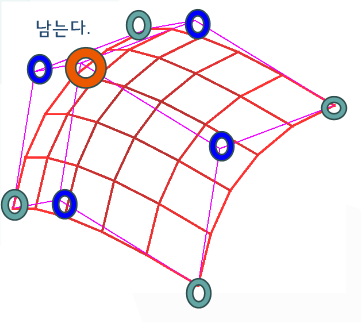
\includegraphics[width=.5\textwidth]{22BS}
	\caption{$(2,2)$-차 베지어 곡면}
	\small $(2,2)$-차 베지어 곡면은 네 모서리가 결정되면 하나의 조절점만 정할 수 있다. 
\end{figure}

$\mathbf{b}_{11}$을 구하기 위해 최소제곱법을 이용한다. 

\subsection{오차함수}
작년 연구에서는 오차함수로 하우스도르프 거리를 이용했다.
\begin{definition}
	거리공간 $(M, d)$의 공집합아 아닌 두 부분집합 $X, Y$사이의 하우스도르프 거리는 다음과 같이 주어진다.\cite{Munkres}
	\begin{equation} \label{hausdorff}
		d_H(X, Y)=\max\left\{\sup_{x\in X}\inf_{y\in Y} d(x, y), \sup_{y\in Y}\inf_{x\in X} d(x, y)\right\}
	\end{equation}
\end{definition}

하우스도르프 거리는 임의의 거리공간에서 두 집합이 서로 떨어진 정도를 나타낸다는 점에서 오차함수로 적절하다.\cite{last year} 그러나 하우스도르프 거리를 곡면에 적용하기에는 문제점이 많다. 기존에는 두 곡선 사이의 하우스도르프 거리를 구하기 위해 구간을 $N$등분해 점들 사이의 거리를 구했는데, 이 경우 시간복잡도가 $O(N^2)$이 된다. 이번에는 곡선이 아니라 곡면이기에 확인해야 하는 변수가 2배 많아지고, 알고리즘의 시간복잡도가 $O(N^4)$으로 제곱이 된다. 그래서 새로운 오차함수를 정의할 필요가 있다. 

\subsection{RGB 저장}
이 방법이 실제로 적용되기 위해서는 곡면 자체 뿐만 아니라 색도 저장해야 한다. 색은 RGB로 표현되므로 R, G, B를 각각 저장하는 방식으로 진행할 것이다. 이는 곡면을 이루는 각 점에 어떤 실수 값이 대응된 것으로 생각할 수 있다. 곡면을 $\Phi$라 할 때 $f=r, g, b$에 대해 $f:\Phi\rightarrow\mathbb{R}$라 하자. 이제 우리가 만든 베지어 곡면이 충분히 근사되어 $\Phi$로 간주할 수 있고 베지어 곡면이 매개변수 $u, v$에 대해 $\mathbf{x}(u, v)$로 매개화될 때, $f\circ\mathbf{x}:[0, 1]^2\rightarrow\mathbb{R}$을 생각할 수 있다. 이제 $f\circ\mathbf{x}$의 그래프를 하나의 곡면으로 보고 이를 다시 베지어 곡면으로 압축한다. 

$f\circ\mathbf{x}$의 그래프는 닫힌 곡면이 아니므로 근사 방법을 그대로 적용할 수 없다. 또 obj를 근사하는 것과는 다른, 적절한 오차함수가 필요할 것이다. 이번 연구에서 RGB 저장을 실제로 구현하지는 못했다. 그러나 충분히 구현 가능하다고 생각하고, 후속 연구에서 시도해볼 수 있다. 

\section{연구 결과}

\subsection{분할 방법} \label{3.1}
원통형 분할을 하기 앞서 몇 가지 사전 작업이 필요하다. 정점 $\mathbf{P}_k$ 중 가장 거리가 먼 두 정점을 $z$축 위에 올리는 일이다. 원점이 모델 밖에 있으면 같은 $(\theta, z)$에 대해 두 개 이상의 점이 존재할 수 있다. 또는 기울어진 타원체를 생각하면, 거리가 가장 먼 두 점이 $z$축 위에 있는 게 좋다는 걸 알 수 있다. 또한 원기둥의 밑면과 같이 $z$축에 수직인 면이 문제가 될 수 있지만, 이 작업을 통해 이런 문제를 해결할 수 있다. 

가장 거리가 먼 두 점을 $(x_1, y_1, z_1), (x_2, y_2, z_2)$라 하자. 각 정점을 평행이동하여 두 점의 중심이 원점에 오게 한다. 
\begin{equation*}
	\mathbf{P}_k\ \leftarrow\ \mathbf{P}_k - \left(\frac{x_1+x_2}2,\ \frac{y_1+y_2}2,\ \frac{z_1+z_2}2\right)^\intercal
\end{equation*}

이제 $xy$ 회전, $yz$ 회전을 통해 두 점을 $z$축 위로 올린다. 각각 다음과 같다. 
\begin{align*}
	\mathbf{P}_k\ \leftarrow\ \begin{pmatrix}
		x_1 & y_1 & 0 \\ -y_1 & x_1 & 0 \\ 0 & 0 & 1
	\end{pmatrix} \mathbf{P}_k \\
	\mathbf{P}_k\ \leftarrow\ \begin{pmatrix}
		z_1 & 0 & -x_1 \\ 0 & 1 & 0 \\ x_1 & 0 & z_1
	\end{pmatrix} \mathbf{P}_k
\end{align*}

최종적으로 거리가 가장 먼 두 점의 좌표를 $(0, 0, \pm h)$라 한다. \\

$\theta$와 $z$의 범위는 각각 $0\leq \theta <2\pi$, $-h \leq z \leq h$이므로, 원통형 분할을 하면 각 영역은 $\theta_i=2\pi i/2^n,\ z_j=-h+2hj/2^n\ (0\leq i, j < 2^n)$을 경계로 한다. 

\subsection{근사 방법}
$\mathbf{b}_{11}$을 제외한 나머지 8개의 조절점은 이미 구했다. 여기선 $\mathbf{b}_{11}$을 찾는 방법을 연구한다. 최소제곱법을 이용하는 아이디어는 선행 연구를 참조했다.\cite{2021} 최소제곱법을 사용하기 위해서는 obj 파일의 각 정점 $\mathbf{P}_k$에 대응되는 베지어 곡면 위의 점 $\mathbf{x}_k=\mathbf{x}(u_k, v_k)$을 알아야 한다. 이미 알고 있는 8개 조절점에 대한 항을 $\mathbf{y}_k$라 하면 다음과 같이 나타낼 수 있다. 
\begin{equation*}
	\mathbf{x}_k=B_1^2(u_k)B_1^2(v_k)\mathbf{b}_{11}+\mathbf{y}_k
\end{equation*}

이제 $\mathbf{x}_k=\mathbf{P}_k\ (k=1, \cdots, K)$의 제곱오차 $S=\sum_{k=1}^K \| \mathbf{x}_k-\mathbf{P}_k \|^2$를 최소화하기 위해 행렬방정식으로 나타낸다.
\begin{equation*}
	\begin{pmatrix}
		B_1^2(u_1)B_1^2(v_1) \\ B_1^2(u_2)B_1^2(v_2) \\ \vdots \\ B_1^2(u_K)B_1^2(v_K)
	\end{pmatrix} \begin{pmatrix}
	b_{11}^x & b_{11}^y & b_{11}^z
	\end{pmatrix} = \begin{pmatrix}
	P_1^x-y_1^x & P_1^y-y_1^y & P_1^z-y_1^z \\ P_2^x-y_2^x & P_2^y-y_2^y & P_2^z-y_2^z \\ \vdots & \vdots & \vdots \\ P_K^x-y_K^x & P_K^y-y_K^y & P_K^z-y_K^z
	\end{pmatrix}
\end{equation*}

이때 윗첨자 $x, y, z$는 각각 벡터의 $x, y, z$성분을 가르킨다. 이 경우에도 제곱오차는 마찬가지로 $S$이다. $AX=B$ 꼴의 행렬방정식에서 최소제곱오차를 가지는 $\hat{X}$는 $\hat{X}=(A^\intercal A)^{-1}A^\intercal B$로 주어지므로, $\mathbf{b}_{11}$을 다음과 같이 근사할 수 있다. 
\begin{equation} \label{findb11}
	\mathbf{b}_{11}=\dfrac{\sum_{k=1}^K B_1^2(u_k)B_1^2(v_k)(\mathbf{P}_k-\mathbf{y}_k)}{\sum_{k=1}^K (B_1^2(u_k)B_1^2(v_k))^2}
\end{equation}

각 $k$에 대해 $u_k$와 $v_k$의 값을 안다면 \cref{findb11}과 같이 $\mathbf{b}_{11}$을 구할 수 있다. 이제 최적의 $u_k, v_k$를 찾기 위해 뉴턴-랩슨 방법을 이용한다. 뉴턴-랩슨 방법을 적용할 함수는 $\mathbf{x}-\mathbf{P}_k$이다. 즉 현재 $u_{n, k}$와 $v_{n, k}$가 주어질 때, 다음과 같이 $u_{n+1, k}$와 $v_{n+1, k}$를 얻는다. 
\begin{align} \label{rearrangeu}
	u_{n+1, k}&=u_{n, k}-\frac{\mathbf{x}-\mathbf{P}_k}{\partial(\mathbf{x}-\mathbf{P}_k)/\partial u} \bigg|_{u=u_{n, k}} \\
	v_{n+1, k}&=v_{n, k}-\frac{\mathbf{x}-\mathbf{P}_k}{\partial(\mathbf{x}-\mathbf{P}_k)/\partial v} \bigg|_{v=v_{n, k}} \label{rearrangev}
\end{align}

그런데 벡터의 나눗셈은 정의되지 않으므로 이번에도 최소제곱법을 이용한다. 즉 $[\partial(\mathbf{x}-\mathbf{P}_k)/\partial u] \Delta u = \mathbf{x}-\mathbf{P}_k$의 제곱 오차를 최소로 하는 스칼라 $\Delta u$를 선택한다. \\

초기 조건 $u_{0, k}=v_{0, k}=0.5$에 대해 다음 과정을 반복한다. 
\begin{enumerate}
	\item \cref{findb11}에 따라 $\mathbf{b}_{11}$을 구한다. 
	\item \cref{rearrangeu}, \cref{rearrangev}에 따라 새로운 $u_k, v_k$를 구한다. 
\end{enumerate}

실험적으로 위 과정을 20번 반복하면 $u_k$와 $v_k$의 값이 거의 일정했다. 

\begin{figure}[h]
	\centering
	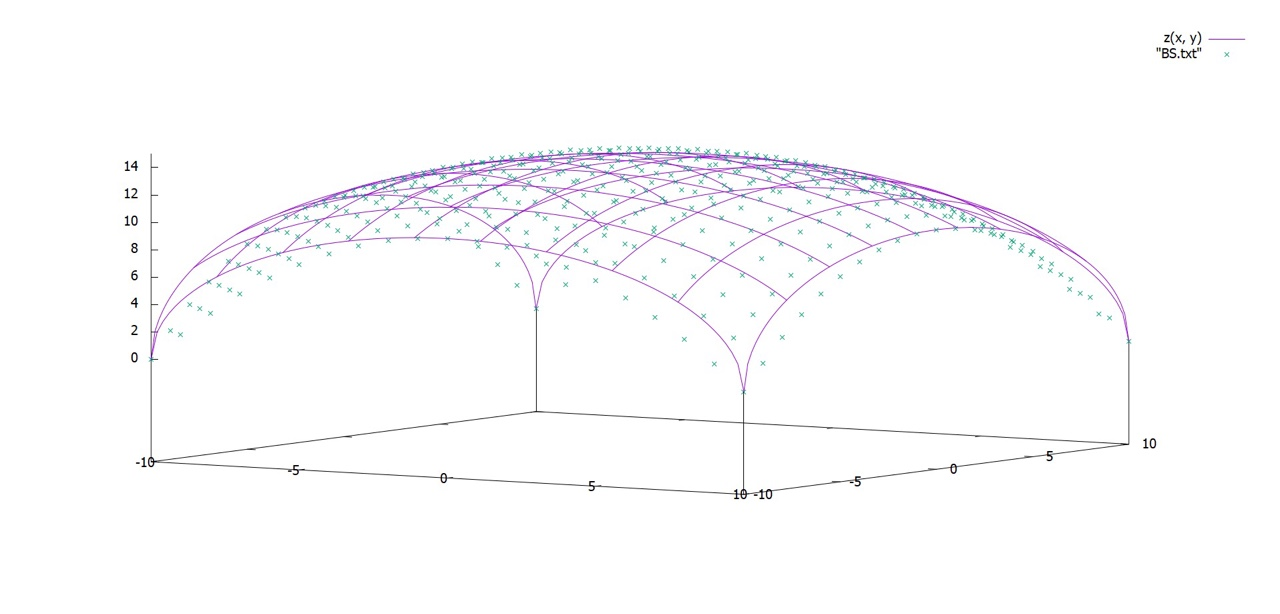
\includegraphics[width=\textwidth]{leastSquare}
	\caption{근사 방법}
	\small 곡면 $z=\sqrt{200-x^2-y^2}\ (-10 \leq x, y \leq 10)$에 위 근사 방법을 적용한 예시이다. 곡면 위 점의 개수는 $K=100$이며 $\mathbf{P}_k$는 $x$와 $y$의 좌표가 $((2i-9)/10,\ (2j-9)/10)\ (i, j = 0, 1, \cdots, 9)$인 점이다. 이때 곡면과 근사한 베지어 곡면 사이의 하우스도르프 거리는 약 6.32이다.
\end{figure}

혹은 최솟값을 얻기 위해 다른 방법도 적용해볼 수 있다. 예를 들어 gradient method도 국소 최솟값을 찾는 하나의 방법이다. 그러나 gradient method는 주어진 3D 모델의 크기에 따라 상수를 바꿔야한다는 단점이 있고, 직접 실험해본 결과 뉴턴-랩슨 방법에 비해 더 나은 결과를 얻지도 못했다. 

\subsection{오차함수}
하우스도르프 거리를 개선하여 다음과 같은 오차함수를 정의하였다. 

\begin{definition}
	분할된 각 영역 내의 점을 $\mathbf{P}_k\ (1\leq k\leq K)$라 하고, 이에 대응되는 베지어 곡면 위의 점을 $\mathbf{x}(u_k, v_k)=\mathbf{x}_k$라 하자. 이때 오차함수 $\mu$는 다음과 같이 주어진다.
	\begin{equation} \label{error}
		\mu=\max_{\text{각 영역}}\max_{1\leq k\leq K} \| \mathbf{x}_k-\mathbf{P}_k \|
	\end{equation}
\end{definition}

$\mathbf{P}_k$와 가장 가까운 베지어 곡면 위의 점이 $\mathbf{x}_k$라는 가정 하에 \cref{hausdorff}를 다시 쓴 것이다. 근사 방법을 생각해보면 충분히 타당한 가정이다. 또한 위 오차함수를 계산하는데 필요한 시간은 전체 점의 개수 $N$에 대해 $O(N)$으로 주어진다. 하우스도르프 거리의 시간 복잡도가 $O(N^2)$인 것과 비교해 더 효율적이다. 

우리는 $n\to\infty$에 따라 $\mu\to0$임을 보였다. 

\begin{figure}[h]
	\centering
	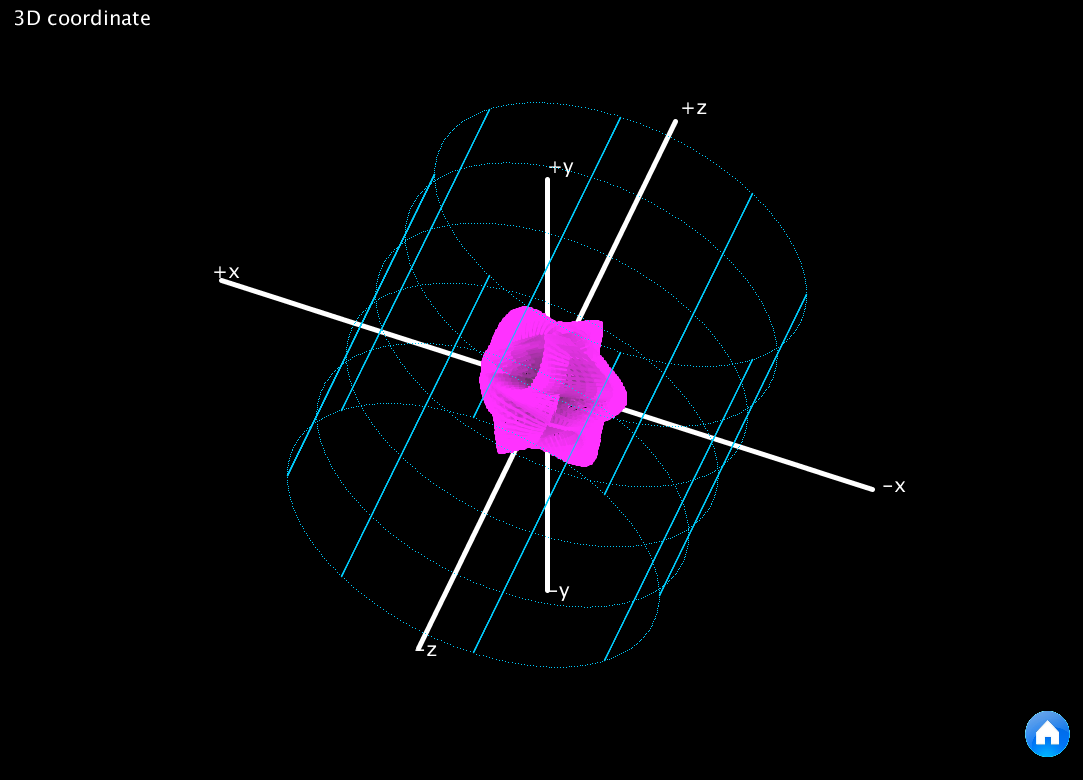
\includegraphics[width=\textwidth]{gg}
	\caption{구면 근사}
	\small 반지름 64인 구면은 근사한 모델(분홍색)로, \cref{error}로 정의한 오차함수는 $\mu<10$이다. 
\end{figure}

\subsection{충분한 근사 가능성}
\begin{theorem}
	위와 같은 근사 방법에 따라 3D 모델을 근사했다고 하자. \cref{error}로 주어진 오차함수 $\mu$에 대해 다음이 성립한다.
	\begin{equation*}
		\lim_{n\to\infty}\mu=0
	\end{equation*}
\end{theorem}

\begin{proof}
	실제로는 $n$이 매우 커지면 어떤 영역 내 $\mathbf{P}_k$가 전혀 없을 수 있다. 이런 문제를 해결하기 위해 $\mathbf{P}_k$가 무수히 많다고 가정한다. 
	
	임의의 양수 $\varepsilon$에 대해 $n \geq N_k$이면 $\| \mathbf{x}_k-\mathbf{P}_k \| < \varepsilon$이 성립하는 자연수 $N_k$가 존재함을 보이자. $\| \mathbf{x}_k-\mathbf{P}_k \| < \| \mathbf{x}_k-\mathbf{b}_{00} \| + \| \mathbf{P}_k-\mathbf{b}_{00} \|$이므로 우변의 두 항이 각각 $\varepsilon/2$보다 작게 만들 수 있음을 보일 것이다. 
	
	우선 $\| \mathbf{P}_k - \mathbf{b}_{00} \|$ 에서 $\mathbf{P}_k$와 $\mathbf{b}_{00}$는 모두 obj파일로 주어진 원 곡면 위의 점이다. $\mathbf{P}_k$의 곡면 위 어떤 근방이 $r$축을 포함하는 평면에 포함되지 않으면 $\| \mathbf{P}_k - \mathbf{b}_{00} \|$의 값을 충분히 작게 만들 수 있다. 또한 그렇지 않은 경우는 \cref{3.1}의 사전 작업에 의해 불가능하다. (그림으로 설명) 따라서 $n \geq N_{k1}$이면 $\| \mathbf{P}_k - \mathbf{b}_{00} \| < \varepsilon/2$인 자연수 $N_{k1}$이 존재한다.
	
	이제 $\| \mathbf{x}_k-\mathbf{b}_{00} \| = \| \mathbf{x}(u_k, v_k) - \mathbf{x}(0, 0) \|$를 살펴보자. $\mathbf{x}_k$가 $\mathbf{P}_k$를 근사한 점이고, 또 $u_k$와 $v_k$의 초기값이 $1/2$이므로 $\mathbf{x}_k$가 영역 안에 있다고 생각할 수 있다. 따라서 $\mathbf{x}_k-\mathbf{b}_{00}$의 $r$축에 수직인 성분은 $n$이 커짐에 따라 $0$에 수렴한다. 또한  $\mathbf{P}_k-\mathbf{b}_{00}$와 같은 논의로 $\mathbf{x}_k-\mathbf{b}_{00}$의 $r$ 성분도 0에 수렴함을 알 수 있다. 따라서 $n \geq N_{k2}$이면 $\| \mathbf{x}_k - \mathbf{b}_{00} \| \leq \varepsilon/2$인 $N_{k2} \in \mathbb{N}$이 존재한다. 
	
	이제 $N_k=\max(N_{k1}, N_{k2})$라 하자. 그러면 $n\geq N_k$일 때 $\| \mathbf{x}_k-\mathbf{P}_k \| < \| \mathbf{x}_k-\mathbf{b}_{00} \| + \| \mathbf{P}_k-\mathbf{b}_{00} \| < \varepsilon$이다. 다시 $N$을 모든 $N_k$들의 최댓값으로 정의하면 $n \geq N \implies \mu < \varepsilon$을 얻는다. 
\end{proof}

\section{결론}
본 연구에서 obj파일로 정점들의 집합과 곡면을 이루는 다각형 면들이 주어졌을 때 베지어 곡면을 이용해 원 곡면을 근사한다. 이를 위해 정점들을 원통형으로 분할하며, 분할된 각 영역에 대해 베지어 곡면의 성질과 Möller–Trumbore intersection algorithm, 최소제곱법, 뉴턴-랩슨 방법을 이용해 베지어 곡면을 구성하는 조절점을 얻는다. 더욱이 제시된 방법에 따라 연구 대상으로 하는 곡면들이 모두 충분히 근사될 수 있음을 보였다. 

실제로 반지름의 길이가 64인 구면에 제시한 방법을 적용했을 때, 실행 시간 1분 이내에 오차함수 $\mu<10$을 얻었고 곡면을 저장하는 메모리는 200배 이상 감소되었다. 

베지어 곡면은 삼각형 분할에 비해 더 효율적이며, 적은 메모리를 요구한다. 그렇기에 본 연구는 VR, AR 등 곡면에 대한 그래픽 기술을 다루는 분야에서의 활용이 기대되며 특히 CAGD 분야에 있어 의미있는 결과이다. 또한 기존에 3D 모델을 저장하기 위해 자주 사용되는 obj파일을 변환시키는 연구이기에 3D 모델링이 필요한 보다 다양한 분야와 접목시킬 수 있다. \\

%%%%%%%%%%%%%%%%%%%%%%%%%%
%%%%%%%%지원 현황%%%%%%%%%
%%%%%%%%%%%%%%%%%%%%%%%%%%

\noindent\fbox{%
    \parbox{\textwidth}{%
    \textbf{
이 보고서는 \researchyearwrite학년도 경기과학고등학교 자율연구의 지원을 받아 제작되었습니다.
}
    }%
}

%%%%%%%%%%%%%%%%%%%%%%%%%%
%%%%%%%%참고 문헌%%%%%%%%%
%%%%%%%%%%%%%%%%%%%%%%%%%%

\begin{thebibliography}{99}
	
\bibitem{Farin} Farin, G. E., \& Farin, G. (2002). \emph{Curves and surfaces for CAGD: a practical guide}. Morgan Kaufmann.

\bibitem{raytriangle} Möller, T., \& Trumbore, B. (1997). Fast, minimum storage ray-triangle intersection. \emph{Journal of graphics tools}, 2(1), 21-28.

\bibitem{last year} 윤상, 박건호. (2020). \emph{Bezier curve를 이용한 3차원 곡선의 애니메이션화} (기초 R\&E). 경기과학고등학고.

\bibitem{Munkres} Munkres, J. (2014). \emph{Topology}. Pearson Education.

\bibitem{2021} Lifton, J. J., Liu, T., \& McBride, J. (2021). Non-linear least squares fitting of Bézier surfaces to unstructured point clouds. \emph{AIMS Mathematics}, 6(4), 3142-3159.

\end{thebibliography}

\end{document}
